\section{Conclusioni}
\begin{frame}
	\frametitle{Conclusioni}
	
	Alla luce dei risultati ottenuti:
	\begin{itemize}
		\justifying
		\item il presente studio evidenzia il valore aggiunto del nuovo modello proposto nel campo della modellazione funzionale spazio-temporale, distinguendosi dal modello f-HDGM grazie all'introduzione del parametro di interazione spaziale $\rho$;
		\item una delle limitazioni riguarda il processo di stima del nuovo parametro in quanto la cross validazione richiede risorse computazionali significative;
		\item è necessaria la modifica dell'algoritmo EM affinché sia in grado di massimizzare la funzione di verosimiglianza $-2\ln L(\boldsymbol{\theta}; Y, Z, X)$, tuttavia ciò richiede ulteriori approfondimenti per risolvere questioni ancora aperte, come lo studio dell'identificabilità del modello.
	\end{itemize}	
\end{frame}

\begin{frame}
	
	\begin{columns}
		\begin{column}{0.5\linewidth}
			Infine:
			\begin{itemize}
				\justifying
				\item per migliorare l'analisi sul bike sharing, si potrebbe considerare l'utilizzo di un dataset pluriennale per catturare la componente stagionale del fenomeno e l'adozione di variazioni metodologiche come il clustering dei punti di ritiro per permettere la stima di modelli spazio-temporali locali, riducendo l'assunzione che il parametro $\rho$ sia spazio-invariante.
			\end{itemize}
		\end{column}
	
		\begin{column}{0.5\linewidth}
			\centering
			\begin{figure}
				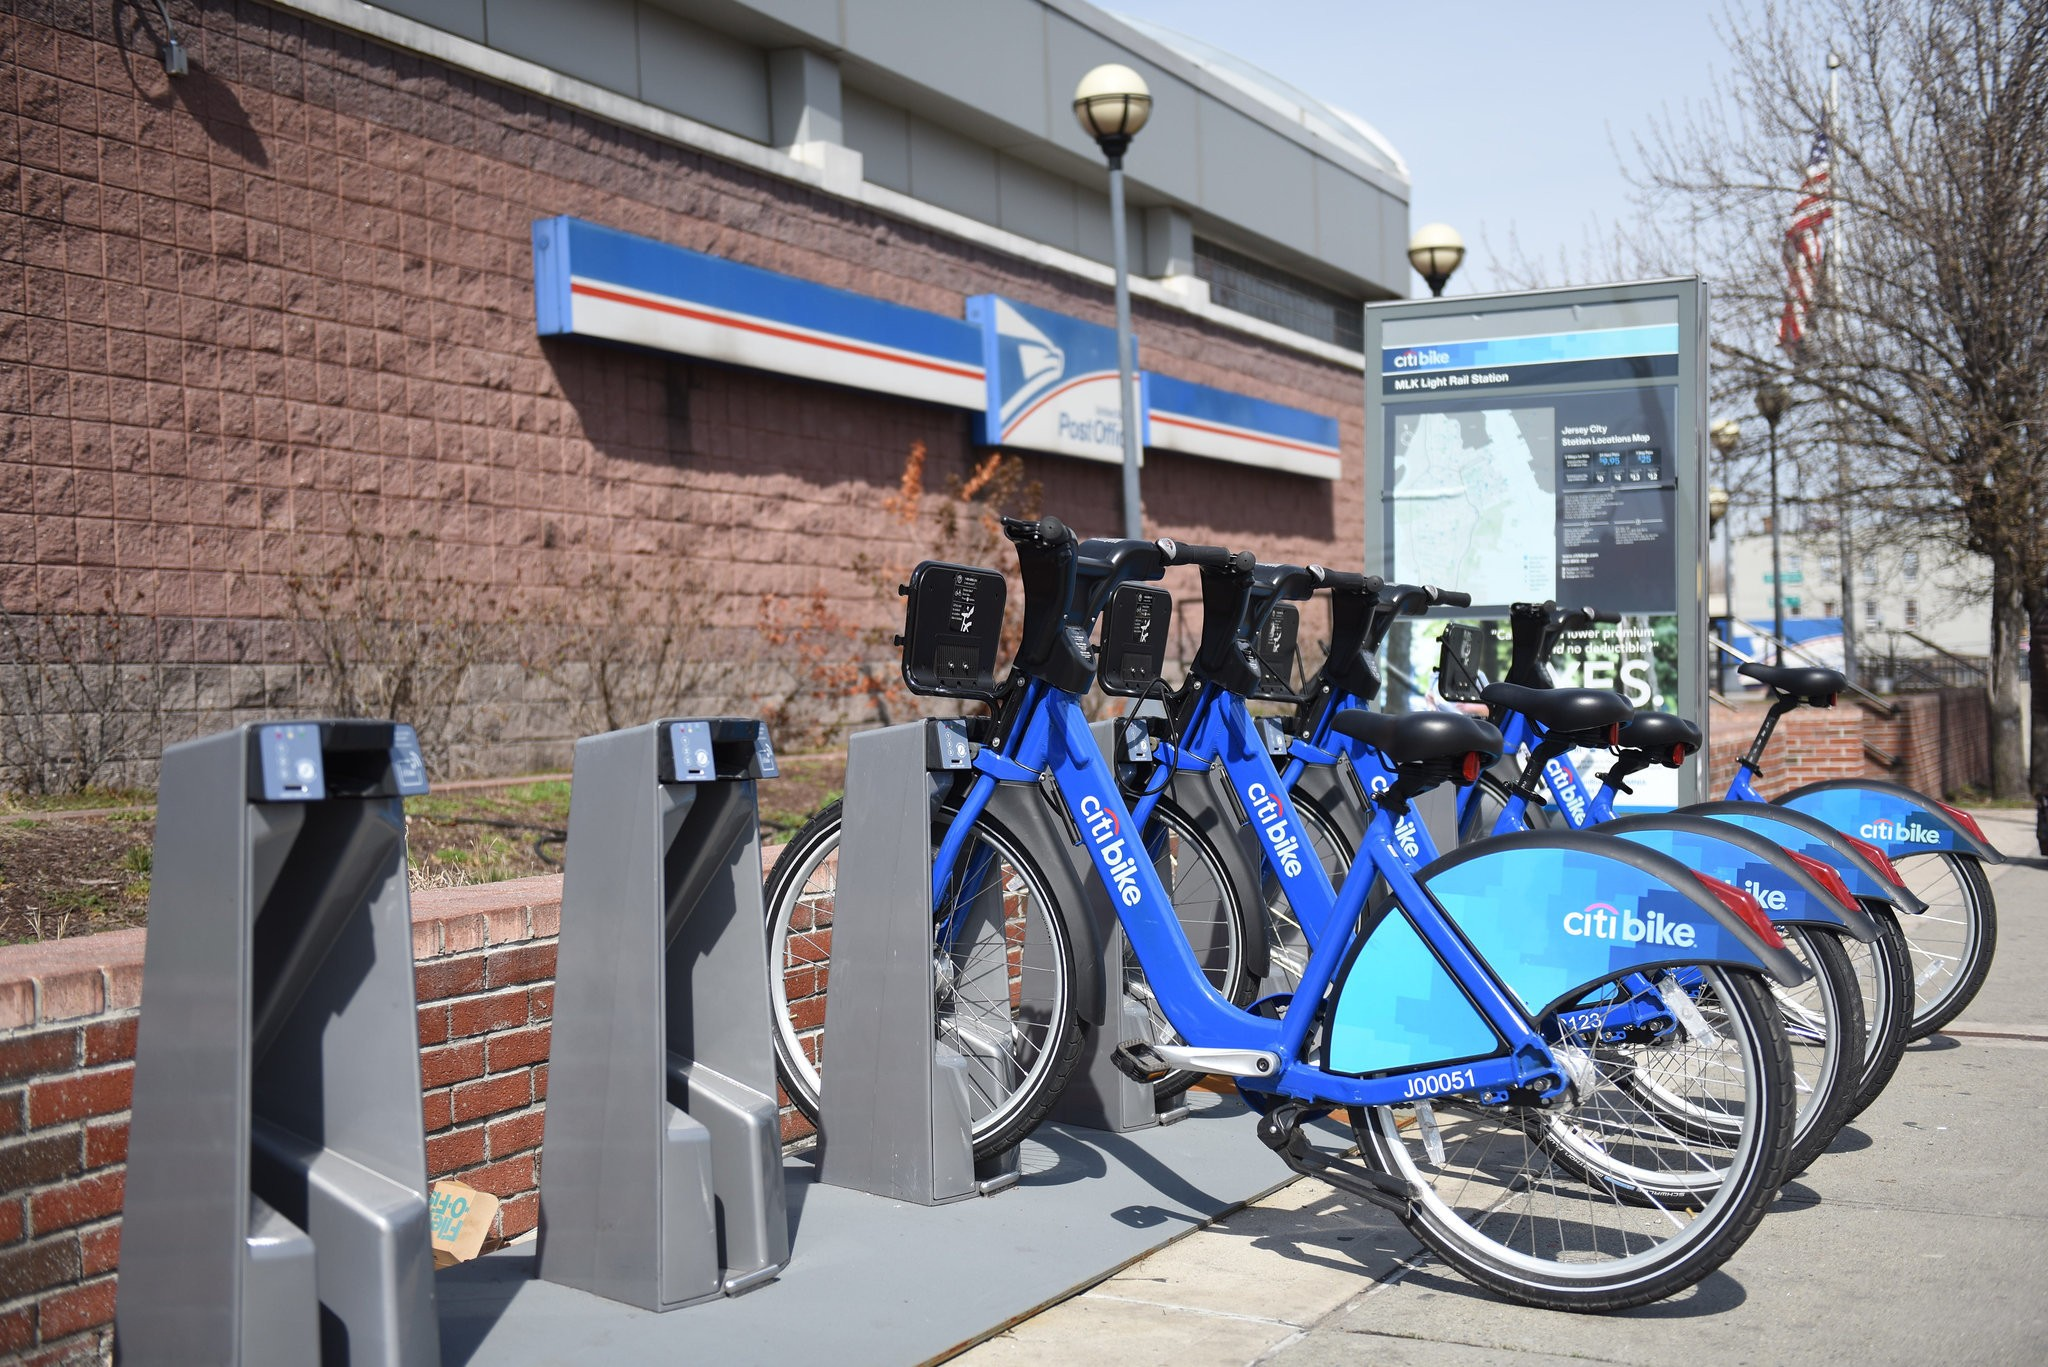
\includegraphics[width=0.95\textwidth]{../Tesi/Immagini/4. Caso di studio/Introduzione/Citi Bike}
			\end{figure}
		\end{column}
	\end{columns}

	\centering
	\vspace{25pt}
	\textbf{Grazie per l'attenzione}
\end{frame}